\documentclass{standalone}
\usepackage{tikz}

\usetikzlibrary{calc,math}

\begin{document}

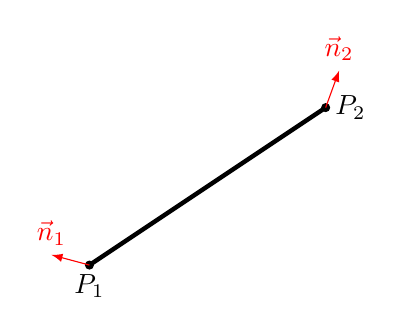
\begin{tikzpicture}
  \coordinate (p1) at (0,0);
  \coordinate (p2) at (3,2);

  \draw[fill] (p1) circle [radius=.05cm] node[below] {$P_1$};
  \draw[fill] (p2) circle [radius=.05cm] node[right] {$P_2$};
  \draw[ultra thick] (p1) -- (p2);

  \draw[red,-latex] (p1) -- ++(165:0.5) node[above] {$\vec{n}_1$};
  \draw[red,-latex] (p2) -- ++(70:0.5)  node[above] {$\vec{n}_2$};
\end{tikzpicture}

\end{document}